\documentclass[withoutpreface]{cumcmthesis}

\usepackage{url}
\usepackage{subcaption}
\usepackage{booktabs}
\usepackage{longtable}
\usepackage{graphicx}

\title{轨道交通大小交路与列车时刻表示例研究}
\tihao{B}
\baominghao{0000}
\schoolname{Research Copy}
\membera{Member A}
\memberb{Member B}
\memberc{Member C}
\supervisor{}
\yearinput{2026}
\monthinput{07}
\dayinput{07}

\begin{document}

\maketitle

\begin{abstract}
本文给出一个面向数模论文生成器的轨道交通时刻表类题目示例。示例并非真实赛题数据，而是用于验证“客流分析--大小交路方案--多目标权衡--时刻表生成--可行性审查--运营建议”的完整链路。首先，根据合成的断面客流识别高峰拥挤区段，并枚举小交路起终点与大小交路列车数。其次，将运营成本拆分为固定发车成本、列车公里成本和车辆使用成本，将服务水平表示为候车时间与拥挤度惩罚的组合，并用归一化综合评分选择候选方案。结果选出小交路覆盖第4站至第10站，大交路12列、小交路13列，重叠区段综合发车间隔为144秒。最后，根据运行时间、停站时间和最小追踪间隔生成完整时刻表，并输出断面容量、追踪间隔、停站时间和场景分析审查表。审查结果显示，示例方案最小容量裕度为4600人次/小时，最小追踪间隔为144秒，最大停站时间为20.4秒。本文的目标是提供一个可复用的研究型生成模板，而不是给出真实运营结论。

\keywords{轨道交通\quad 大小交路\quad 列车时刻表\quad 断面客流\quad 可行性审查}
\end{abstract}

\section{问题重述}

城市轨道交通高峰期通常存在明显的客流空间不均衡现象：中心区段断面客流较高，外围区段客流较低。如果全线均采用同一发车频率，容易造成中心区段运能不足或外围区段运能浪费。大小交路运营通过在高需求区段增开短交路列车，在保持全线基本服务的同时提高核心区段运能，是轨道交通运营优化中的常见策略。

本示例研究一个12站单向高峰线路。已知各相邻车站区间的断面客流、区间运行时间、区间长度、列车定员、发车间隔上下界、停站时间上下界和最小追踪间隔。需要完成以下任务：

\begin{enumerate}
\item 设计大交路与小交路组合运营方案，确定小交路起终点以及大小交路列车数；
\item 在所选运营方案下生成等间隔列车时刻表；
\item 审查断面运能、追踪间隔和停站时间是否满足约束；
\item 对需求变化和发车间隔变化进行场景分析，给出运营建议。
\end{enumerate}

\section{问题分析}

本题具有典型的“运营方案--时刻表--审查建议”链路。第一问本质上是离散服务模式选择问题：小交路起终点和列车数均为离散变量，可通过候选方案枚举形成可行集，再依据成本与服务水平进行排序。第二问是运行图生成问题，必须把第一问的列车数和小交路区间转化为各站到发时刻。第三问不是简单描述性建议，而应基于容量、追踪、停站和场景实验给出可量化解释。

因此，本文采用如下建模路线：

\[
\begin{aligned}
\text{断面客流} &\rightarrow \text{候选大小交路}
\rightarrow \text{成本/服务评价}\\
&\rightarrow \text{时刻表递推}
\rightarrow \text{可行性审查}
\rightarrow \text{场景建议}.
\end{aligned}
\]

该路线与项目知识库中的 Type I 轨道交通时刻表范式一致，重点不是只画出运行图，而是保存可机器审查的完整产物。

\section{基本假设}

\begin{enumerate}
\item 示例线路为单方向高峰小时，暂不考虑上下行交互和车辆回库接续。
\item 断面客流代表该小时内各区间最大服务需求，列车定员为固定值。
\item 大交路服务全线，小交路仅服务高需求区段。
\item 停站时间由基础时间和乘客交换量估计，并限制在给定上下界内。
\item 本示例数据为合成数据，只用于验证生成器流程，不用于真实运营决策。
\end{enumerate}

\section{符号说明}

\begin{table}[H]
\centering
\caption{主要符号说明}
\label{tab:rail-symbols}
\begin{tabular}{cl}
\toprule
符号 & 含义 \\
\midrule
$i$ & 车站或区间编号 \\
$k$ & 列车编号 \\
$q_i$ & 第$i$个区间断面客流 \\
$C$ & 单列车定员 \\
$n_B,n_S$ & 大交路和小交路列车数 \\
$h$ & 重叠区段综合发车间隔 \\
$a_{k,i},d_{k,i}$ & 第$k$列车在第$i$站的到达、出发时刻 \\
$r_i$ & 第$i$个区间运行时间 \\
$\tau_{k,i}$ & 第$k$列车在第$i$站停站时间 \\
\bottomrule
\end{tabular}
\end{table}

\section{数据处理与客流特征}

示例数据包含12个车站和11个相邻区间。断面客流分布如图~\ref{fig:rail-section-flow}所示，中部区段客流显著高于两端区段。这一结构适合采用小交路加密服务：外围区段由大交路保证基本服务，中心重叠区段由大交路和小交路共同提供运能。

\begin{figure}[H]
\centering
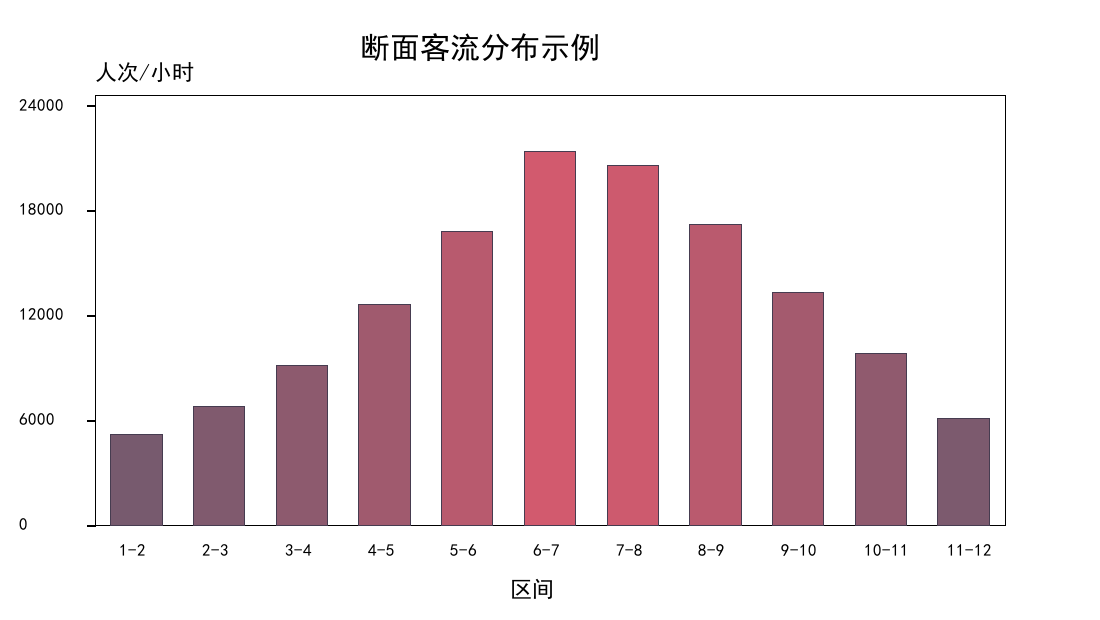
\includegraphics[width=0.90\textwidth]{figures/rail_section_flow.png}
\caption{合成线路断面客流分布}
\label{fig:rail-section-flow}
\end{figure}

\section{模型建立}

\subsection{候选运营方案}

设小交路覆盖车站$s$至$e$。对每一个候选$(s,e)$，分别计算大交路独立区段和大小交路重叠区段的最小列车数。容量约束为
\[
n_B C \geq \max_{i\notin [s,e)} q_i,
\]
\[
(n_B+n_S)C \geq \max_{i\in [s,e)} q_i.
\]

发车间隔约束为
\[
120 \leq \frac{3600}{n_B+n_S} \leq 360,\quad
\frac{3600}{n_B}\leq 360.
\]

为避免生成不便执行的混乱车序，示例中还要求大小交路列车数比例接近$1:1$、$1:2$、$2:1$或$3:1$等易编排比例。

\subsection{成本与服务目标}

运营成本分为固定发车成本、列车公里成本和车辆使用成本：
\[
F=18(n_B+n_S),
\]
\[
V=2.6\cdot 2(n_BL_B+n_SL_S),
\]
\[
G=35(n_B+n_S),
\]
其中$L_B$和$L_S$分别表示大交路和小交路单程长度。总成本为
\[
Z_1=F+V+G.
\]

服务水平综合考虑平均候车时间和拥挤度惩罚：
\[
Z_2=\frac{h}{2}+160\rho,
\]
其中$\rho$为各区段客流与服务能力之比的最大值。对$Z_1$和$Z_2$归一化后，采用加权评分
\[
S=0.52\hat{Z}_1+0.48\hat{Z}_2
\]
选择综合评分最小的候选方案。

\subsection{列车时刻表递推}

对第$k$列车和第$i$站，到发时刻递推为
\[
a_{k,i}=d_{k,i-1}+r_{i-1},
\]
\[
\tau_{k,i}=\min\{\tau_{\max},\max(\tau_{\min},14+0.16p_{k,i})\},
\]
\[
d_{k,i}=a_{k,i}+\tau_{k,i}.
\]
同时加入最小追踪间隔约束：
\[
d_{k,i}\geq d_{k-1,i}+105.
\]
当递推结果不满足追踪间隔时，自动推迟当前列车在对应车站的出发时刻。

\section{求解过程}

程序首先枚举小交路起终点和大小交路列车数，剔除容量、发车间隔和比例不满足要求的方案；然后计算每个可行方案的成本、服务指标和综合评分；最后对最优方案生成时刻表，并输出容量、追踪和停站审查文件。候选运营方案前五名见表~\ref{tab:rail-operation-candidates}。

\begin{table}[H]
\centering
\caption{轨道交通候选运营方案前五名}
\label{tab:rail-operation-candidates}
\small
\begin{tabular}{ccccrrrr}
\toprule
排名 & 小交路 & 大交路 & 小交路 & 总间隔(s) & 成本 & 服务指标 & 综合分 \\
\midrule
1 & 4-10 & 12 & 13 & 144.0 & 2681.2 & 186.1 & 0.4026 \\
2 & 4-10 & 12 & 12 & 150.0 & 2588.6 & 193.9 & 0.4054 \\
3 & 4-10 & 11 & 11 & 163.6 & 2372.9 & 211.5 & 0.4092 \\
4 & 4-10 & 13 & 13 & 138.5 & 2804.4 & 179.0 & 0.4141 \\
5 & 4-10 & 13 & 14 & 133.3 & 2896.9 & 172.3 & 0.4164 \\
\bottomrule
\end{tabular}
\end{table}


图~\ref{fig:rail-cost-service}展示了候选方案的成本--服务水平权衡。红色点为选定方案。该图的作用不是替代数学模型，而是帮助检查所选方案是否处在合理的权衡区域。

\begin{figure}[H]
\centering
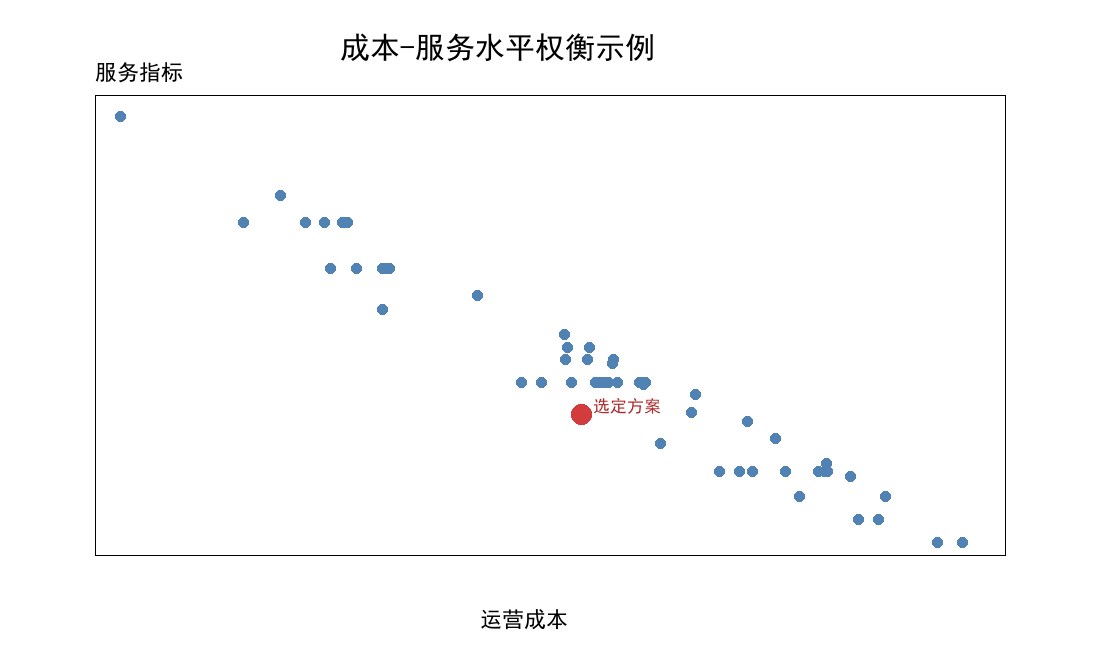
\includegraphics[width=0.88\textwidth]{figures/rail_cost_service_tradeoff.png}
\caption{候选方案成本--服务水平权衡}
\label{fig:rail-cost-service}
\end{figure}

\section{结果与分析}

综合评分最小的方案为小交路覆盖第4站至第10站，大交路12列，小交路13列，重叠区段综合发车间隔为144秒。该方案在中心高客流区段通过大小交路叠加提供较高频率，而两端区段保留大交路贯通服务。

完整时刻表以机器可读文件保存于\texttt{runs/rail-demo/rail\_full\_timetable.csv}。正文中节选部分车次与车站到发时刻见表~\ref{tab:rail-timetable-sample}。

\begin{table}[H]
\centering
\caption{列车时刻表节选}
\label{tab:rail-timetable-sample}
\small
\begin{tabular}{cclccc}
\toprule
车次 & 类型 & 车站 & 到达 & 出发 & 停站(s) \\
\midrule
T01 & 小交路 & 站4 & 07:06:45 & 07:07:05 & 20 \\
T01 & 小交路 & 站5 & 07:08:50 & 07:09:10 & 20 \\
T01 & 小交路 & 站6 & 07:11:30 & 07:11:50 & 20 \\
T01 & 小交路 & 站7 & 07:13:55 & 07:14:15 & 20.4 \\
T01 & 小交路 & 站8 & 07:16:10 & 07:16:30 & 20 \\
T01 & 小交路 & 站9 & 07:18:45 & 07:19:05 & 20 \\
T01 & 小交路 & 站10 & 07:20:50 & 07:21:10 & 20 \\
T02 & 大交路 & 站1 & 07:02:24 & 07:02:44 & 20 \\
T02 & 大交路 & 站2 & 07:04:39 & 07:04:59 & 20 \\
T02 & 大交路 & 站3 & 07:06:39 & 07:06:59 & 20 \\
T02 & 大交路 & 站4 & 07:09:09 & 07:09:29 & 20 \\
T02 & 大交路 & 站5 & 07:11:14 & 07:11:34 & 20 \\
T02 & 大交路 & 站6 & 07:13:54 & 07:14:14 & 20 \\
T02 & 大交路 & 站7 & 07:16:19 & 07:16:39 & 20.4 \\
T02 & 大交路 & 站8 & 07:18:34 & 07:18:54 & 20 \\
T02 & 大交路 & 站9 & 07:21:09 & 07:21:29 & 20 \\
T02 & 大交路 & 站10 & 07:23:14 & 07:23:34 & 20 \\
T02 & 大交路 & 站11 & 07:25:34 & 07:25:54 & 20 \\
T02 & 大交路 & 站12 & 07:27:34 & 07:27:54 & 20 \\
T03 & 小交路 & 站4 & 07:11:33 & 07:11:53 & 20 \\
T03 & 小交路 & 站5 & 07:13:38 & 07:13:58 & 20 \\
T03 & 小交路 & 站6 & 07:16:18 & 07:16:38 & 20 \\
T03 & 小交路 & 站7 & 07:18:43 & 07:19:03 & 20.4 \\
T03 & 小交路 & 站8 & 07:20:58 & 07:21:18 & 20 \\
T03 & 小交路 & 站9 & 07:23:33 & 07:23:53 & 20 \\
T03 & 小交路 & 站10 & 07:25:38 & 07:25:58 & 20 \\
T04 & 大交路 & 站1 & 07:07:12 & 07:07:32 & 20 \\
T04 & 大交路 & 站2 & 07:09:27 & 07:09:47 & 20 \\
\bottomrule
\end{tabular}
\end{table}


根据完整时刻表绘制的运行图见图~\ref{fig:rail-timetable}。蓝色线表示大交路列车，紫色线表示小交路列车。从图中可以看出，小交路列车仅在第4站至第10站之间运行，符合方案设定。

\begin{figure}[H]
\centering
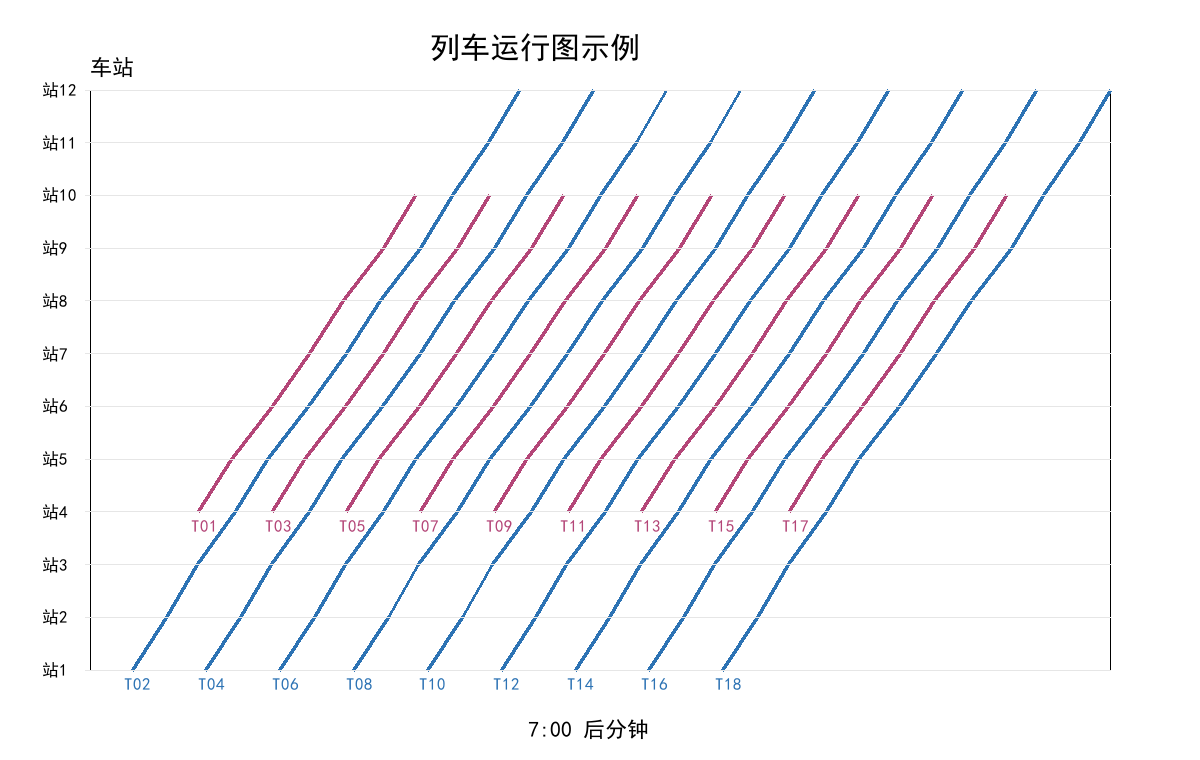
\includegraphics[width=0.92\textwidth]{figures/rail_timetable_diagram.png}
\caption{大小交路列车运行图示例}
\label{fig:rail-timetable}
\end{figure}

\section{可行性审查与场景分析}

容量审查结果见表~\ref{tab:rail-capacity-audit}。所有断面均满足客流需求，最小容量裕度为4600人次/小时。

\begin{table}[H]
\centering
\caption{选定方案断面容量审查节选}
\label{tab:rail-capacity-audit}
\small
\begin{tabular}{crcrrrc}
\toprule
区间 & 客流 & 服务区段 & 列车数 & 能力 & 裕度 & 状态 \\
\midrule
1-2 & 5200 & 大交路独立 & 12 & 14400 & 9200 & Pass \\
2-3 & 6800 & 大交路独立 & 12 & 14400 & 7600 & Pass \\
3-4 & 9100 & 大交路独立 & 12 & 14400 & 5300 & Pass \\
4-5 & 12600 & 大小交路重叠 & 25 & 30000 & 17400 & Pass \\
5-6 & 16800 & 大小交路重叠 & 25 & 30000 & 13200 & Pass \\
6-7 & 21400 & 大小交路重叠 & 25 & 30000 & 8600 & Pass \\
7-8 & 20600 & 大小交路重叠 & 25 & 30000 & 9400 & Pass \\
8-9 & 17200 & 大小交路重叠 & 25 & 30000 & 12800 & Pass \\
9-10 & 13300 & 大小交路重叠 & 25 & 30000 & 16700 & Pass \\
10-11 & 9800 & 大交路独立 & 12 & 14400 & 4600 & Pass \\
11-12 & 6100 & 大交路独立 & 12 & 14400 & 8300 & Pass \\
\bottomrule
\end{tabular}
\end{table}


追踪间隔审查共检查223条相邻列车事件，全部满足105秒的最小追踪间隔；停站时间审查显示，示例中最大停站时间为20.4秒，位于20至60秒的允许范围内。对应的机器可读审查文件保存在\texttt{runs/rail-demo/}目录中。

运营建议不能只停留在文字判断。表~\ref{tab:rail-scenario-analysis}给出了需求变化和发车间隔变化下的场景分析。当需求上浮时，应优先缩短重叠区段间隔或增开小交路；当发车间隔放大导致能力不足时，应回退到更高频率方案。

\begin{table}[H]
\centering
\caption{运营建议场景分析}
\label{tab:rail-scenario-analysis}
\small
\begin{tabular}{lrrrrl}
\toprule
场景 & 最大客流 & 所需列车 & 计划列车 & 间隔(s) & 建议 \\
\midrule
需求0.8倍 & 17120.0 & 15 & 25 & 144.0 & 保持方案 \\
需求0.9倍 & 19260.0 & 17 & 25 & 144.0 & 保持方案 \\
需求1.0倍 & 21400.0 & 18 & 25 & 144.0 & 保持方案 \\
需求1.1倍 & 23540.0 & 20 & 25 & 144.0 & 缩短间隔或增开小交路 \\
需求1.2倍 & 25680.0 & 22 & 25 & 144.0 & 缩短间隔或增开小交路 \\
间隔120s & 21400 & 18 & 30 & 120 & 容量充足 \\
间隔150s & 21400 & 18 & 24 & 150 & 容量充足 \\
间隔180s & 21400 & 18 & 20 & 180 & 容量充足 \\
间隔210s & 21400 & 18 & 17 & 210 & 容量不足 \\
间隔240s & 21400 & 18 & 15 & 240 & 容量不足 \\
\bottomrule
\end{tabular}
\end{table}


\section{模型评价}

本文示例的优点在于产物链完整：从方案候选、时刻表输出到容量和追踪审查均有机器可读文件支撑，便于后续质量审查器逐项核验。与只在正文中展示运行图相比，这种做法更适合长期维护的论文生成器，因为审查器可以直接检查关键约束是否通过。

不足也较明显。第一，数据为合成数据，无法代表真实线路的复杂客流结构。第二，服务水平指标较简化，没有显式建模换乘、站台拥挤和乘客路径选择。第三，车辆周转、折返能力和上下行接续尚未纳入。真实赛题中，应根据附件数据扩展OD分配、车辆运用和折返能力约束。

\section{结论}

本示例验证了轨道交通时刻表类题目的生成器路线：先用断面客流识别小交路需求，再枚举大小交路运营方案，随后依据成本和服务水平选择方案，最后生成完整时刻表并进行容量、追踪、停站和场景审查。示例结果给出小交路第4站至第10站、大交路12列、小交路13列、综合间隔144秒的方案，并生成完整可审查产物。后续应将该路线接入真实赛题附件读取、OD乘客分配和更严格的多目标求解方法。

\begin{thebibliography}{9}
\bibitem{urbanrail}
Vuchic V R. Urban Transit Systems and Technology. Wiley, 2007.
\bibitem{timetable}
Ceder A. Public Transit Planning and Operation: Theory, Modeling and Practice. CRC Press, 2016.
\bibitem{cumcm}
China Society for Industrial and Applied Mathematics. Mathematical modeling contest public materials.
\end{thebibliography}

\begin{appendices}
\section{生成产物清单}
本示例由\texttt{src/rail\_timetable\_demo.py}生成。主要产物包括：
\begin{itemize}
\item \texttt{runs/rail-demo/rail\_operation\_candidates.csv}
\item \texttt{runs/rail-demo/rail\_selected\_operation\_plan.csv}
\item \texttt{runs/rail-demo/rail\_full\_timetable.csv}
\item \texttt{runs/rail-demo/rail\_capacity\_audit.csv}
\item \texttt{runs/rail-demo/rail\_tracking\_audit.csv}
\item \texttt{runs/rail-demo/rail\_dwell\_audit.csv}
\item \texttt{runs/rail-demo/rail\_scenario\_analysis.csv}
\end{itemize}
\end{appendices}

\end{document}
